\section{Exploring the incidents' temporal distribution}

\subsection*{Question 5.1}
\textit{How do the different types of incidents (as represented by Event Clearance Group) vary in number over the different years? Do you see different types of incidents having the same temporal variation pattern over the same year(s)?}

\begin{figure}[h]
	\centering
	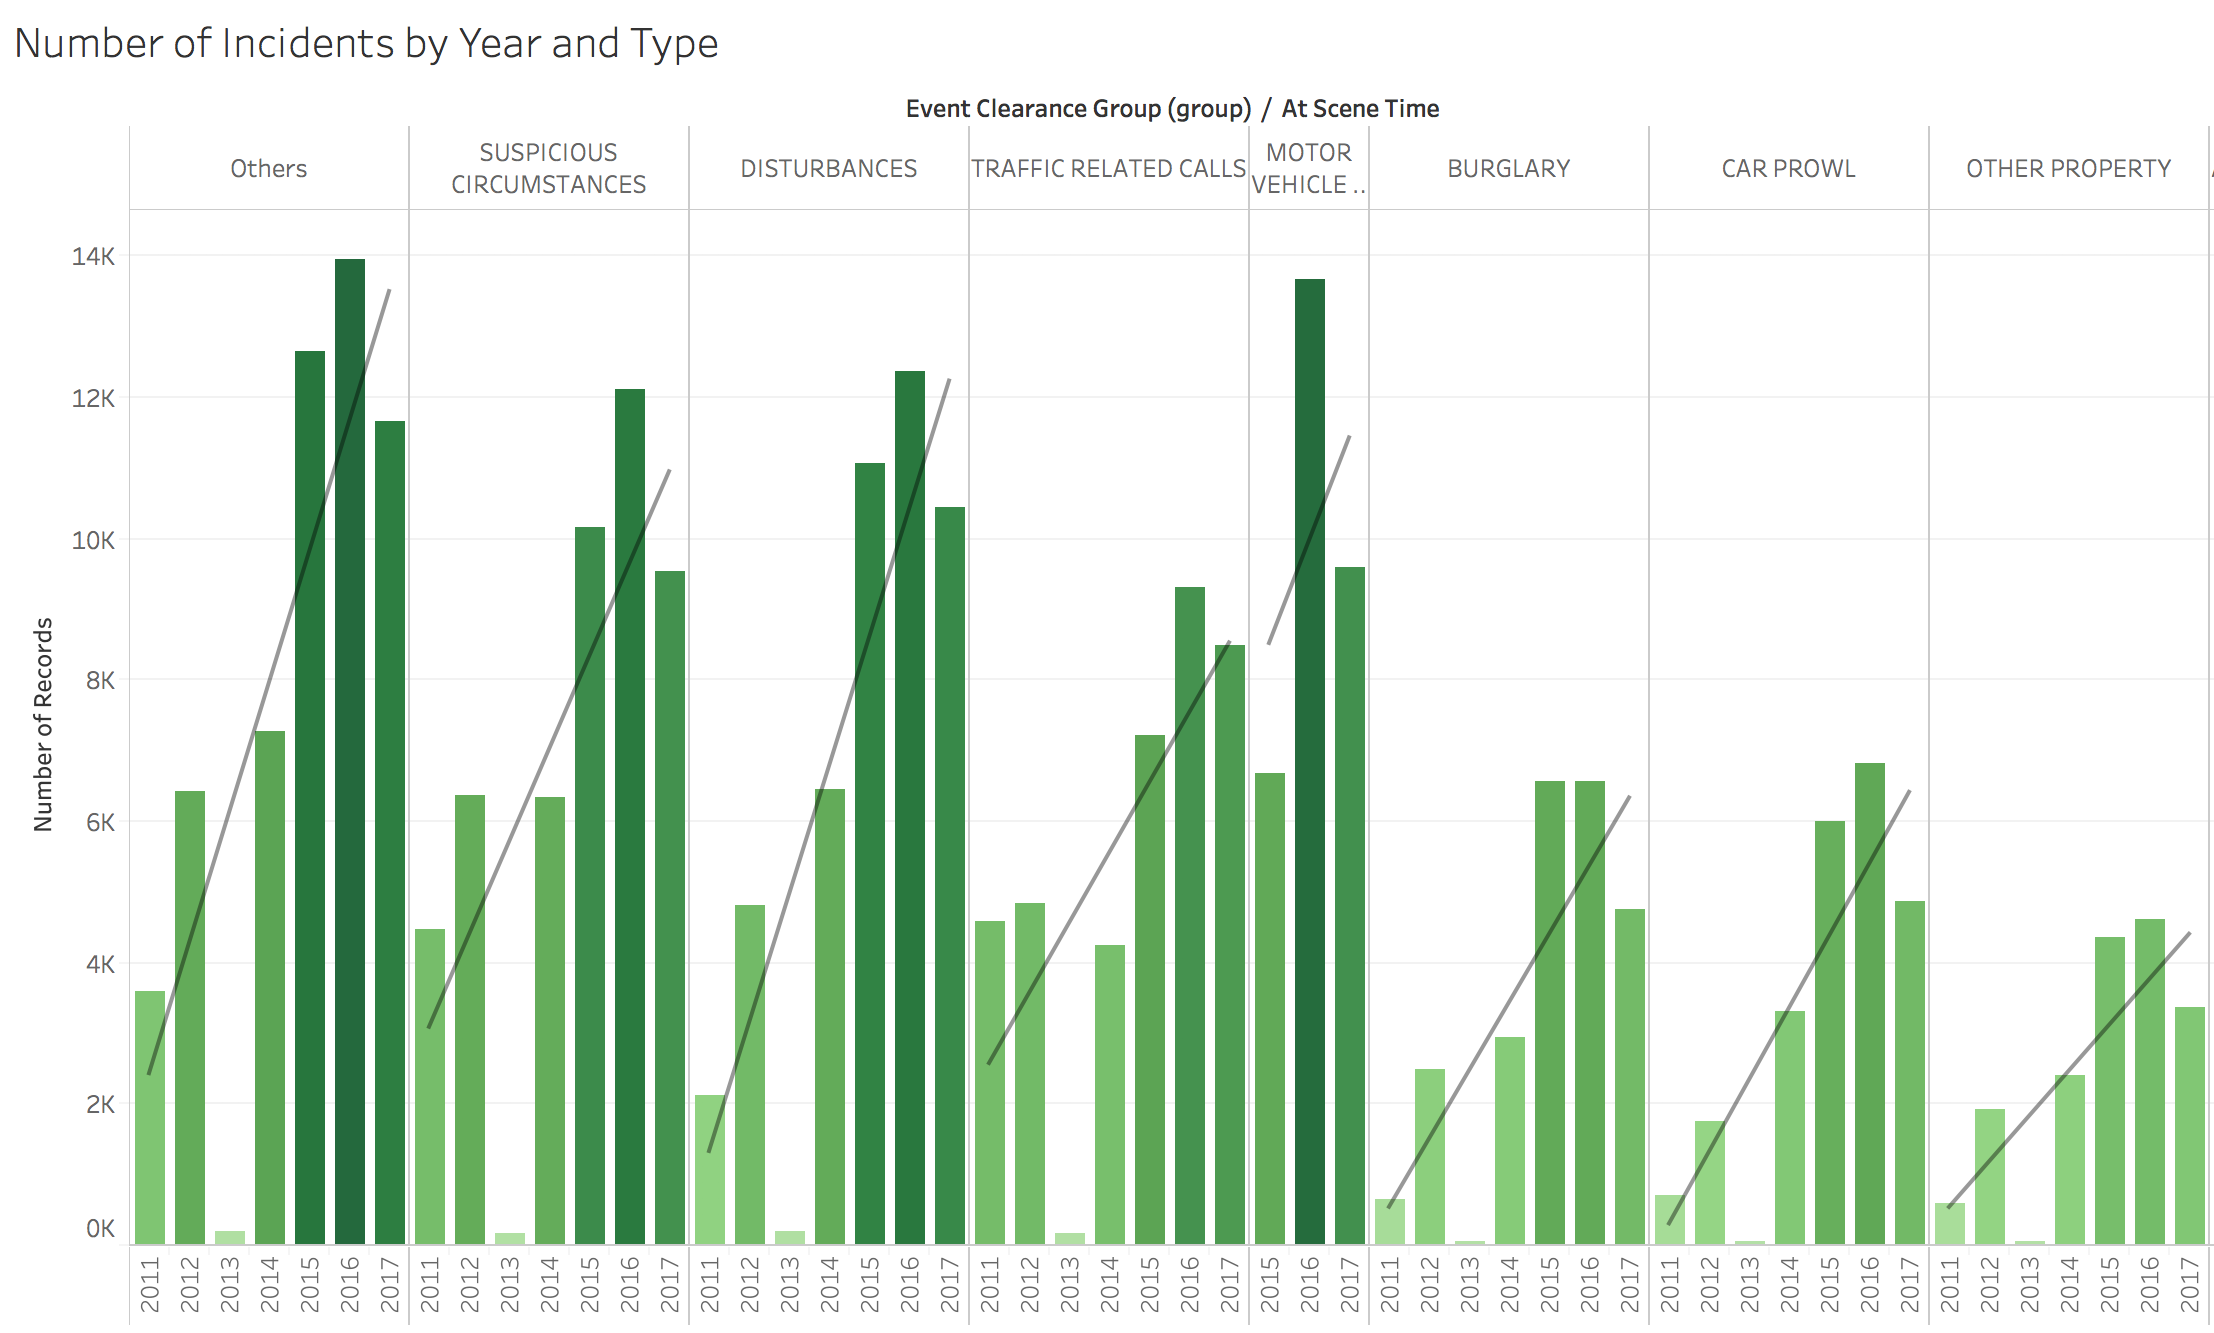
\includegraphics[width=0.9\columnwidth]{figures/5_1_incidents_by_type_and_year}
	\caption{Number of incidents by year and type. The sheet is called \textit{Number of Incidents by Year and Type} in Tableau.}
	\label{fig:5_1_incidents_by_type_and_year}
\end{figure}

The visualization uses bar charts and the small multiple design principle.
The x-axis represent the time (in years), while the y-axis encodes the number of incidents for the given year.
The bar chart is replicated for each incident type; bar charts for different types are organized in columns.
Color is used to overload the encoding of the number of incidents (showed by the y-axis).
Trend lines are drawn for each small bar chart to show the trend of the number of incidents over year for each different type.
The bar charts are ordered for the total number of incidents per type (decreasing).
The types with less incidents are aggregated together in the \textit{Others} group to spare space on the screen and thus better fit the visualization.
Since there are very few data for $2009$ and $2010$, those years are removed from the visualization.
We filter also null values for the date since we are interested in the trend of incidents over years.

\cref{fig:5_1_incidents_by_type_and_year} shows the visualization.
We can observe the following:
\begin{itemize}
    \item Only $2$ incidents' types decreased over time, namely \textit{Accident Investigation} and \textit{Mental Health}. For both types there is no single incident reported in years $2016$ and $2017$. We believe that this might be due to a change in the classification of incidents in types between $2015$ and $2016$.
    \item All other types of incidents showed an increase over time.
    \item Most incidents show a common pattern: there is an increase from $2011$ to $2012$ and a clear drop in $2013$; $2014$ has a about the same number of incidents as $2014$; years $2015$ and $2016$ have a fast increase, with the peak in $2016$; $2017$ has slightly less incidents than $2016$ (this is probably due to the missing data for the last $3$ months of 2017).
\end{itemize}

The visualization allows to answer the question.
However, it does not show the general trend of the incidents number over years.
To solve this problem, we created a second visualization using another bar chart.
The y-axis represents the incidents' types, the x-axis and color encode the number of incidents for the given year.
We use a continuous heatmap for the color, but a different color for the maximum value in comparison with the visualization in \cref{fig:5_1_incidents_by_type_and_year}.

\begin{figure}[h]
	\centering
	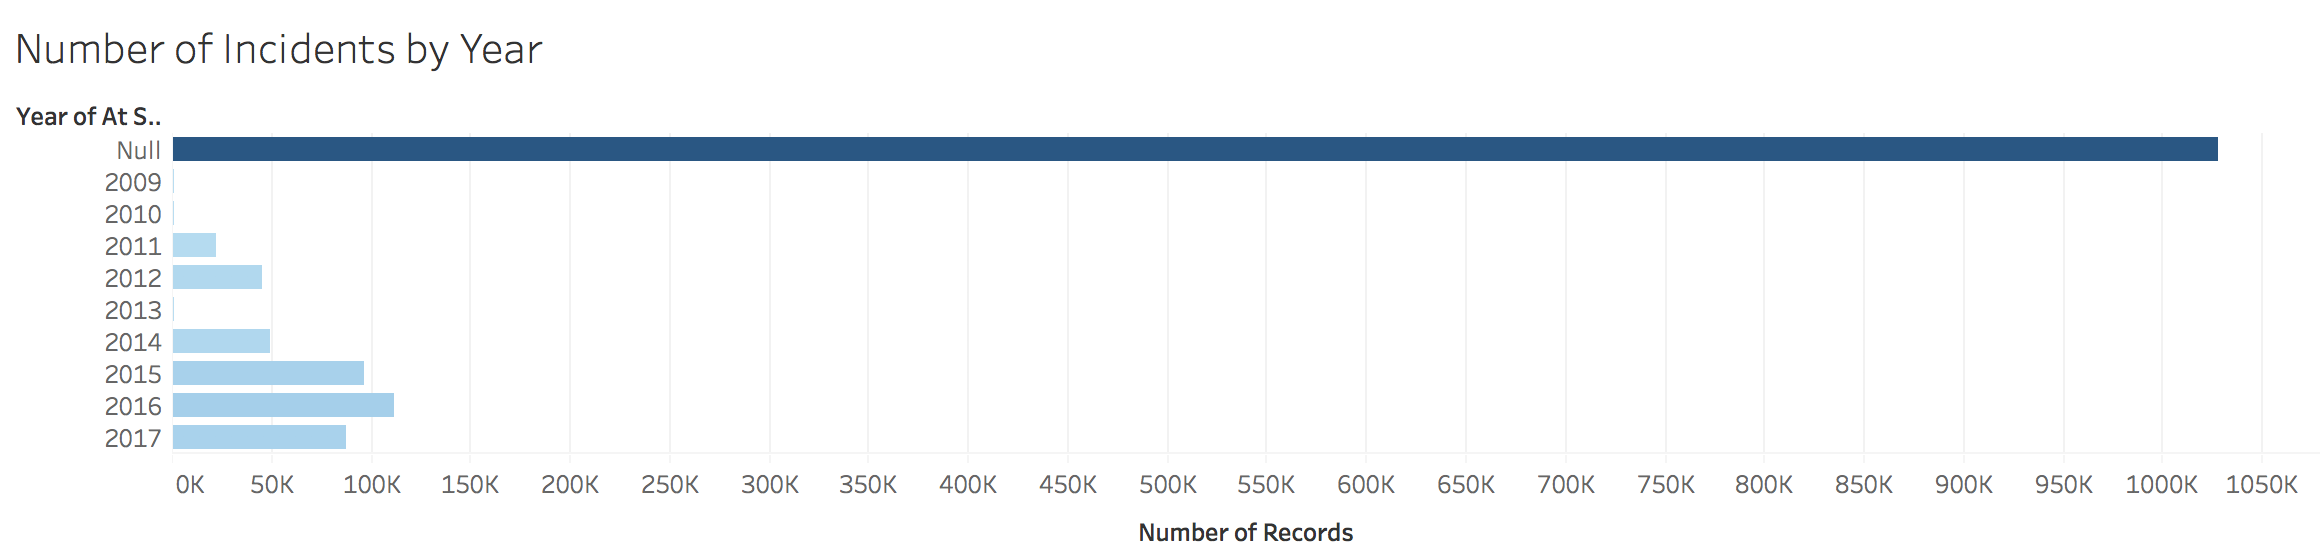
\includegraphics[width=0.9\columnwidth]{figures/5_1_incidents_by_year}
	\caption{Number of incidents by year. The sheet is called \textit{Number of Incidents by Year} in Tableau.}
	\label{fig:5_1_incidents_by_year}
\end{figure}

The visualization is showed in \cref{fig:5_1_incidents_by_year}.
We can notice that:
\begin{itemize}
    \item The majority of incidents in the dataset do not have the date information. The confident of the answer to the question is thus low.
    \item The general temporal distribution of incidents has the same trend of most incidents' types.
\end{itemize} 

The visualizations are grouped together in the \textit{Incidents Temporal Distribution by Type and Year} dashboard.


\subsection*{Question 5.2}
\textit{How do the different types of reported incidents (as represented by Initial Type Group) vary over the 24 hours of a day, for the entire data collection? Are there certain hours having a higher rate of reported incidents?}

The visualization uses bar charts and the small multiple design principle.
For each chart, the y-axis represent the hour of the day, while the x-axis and the color encode the number of incidents for the given hour.
The chart is replicated for each incident type, organized in columns.
The bar charts are ordered for the total number of incidents per type (decreasing, from left to right).
The types with less incidents are aggregated together in the \textit{Others} group to spare space on the screen thus better and fit the visualization and null values are filtered out.
We add the average line for each type in order to easier spot hours with more or less incidents than the average.

\begin{figure}[h]
	\centering
	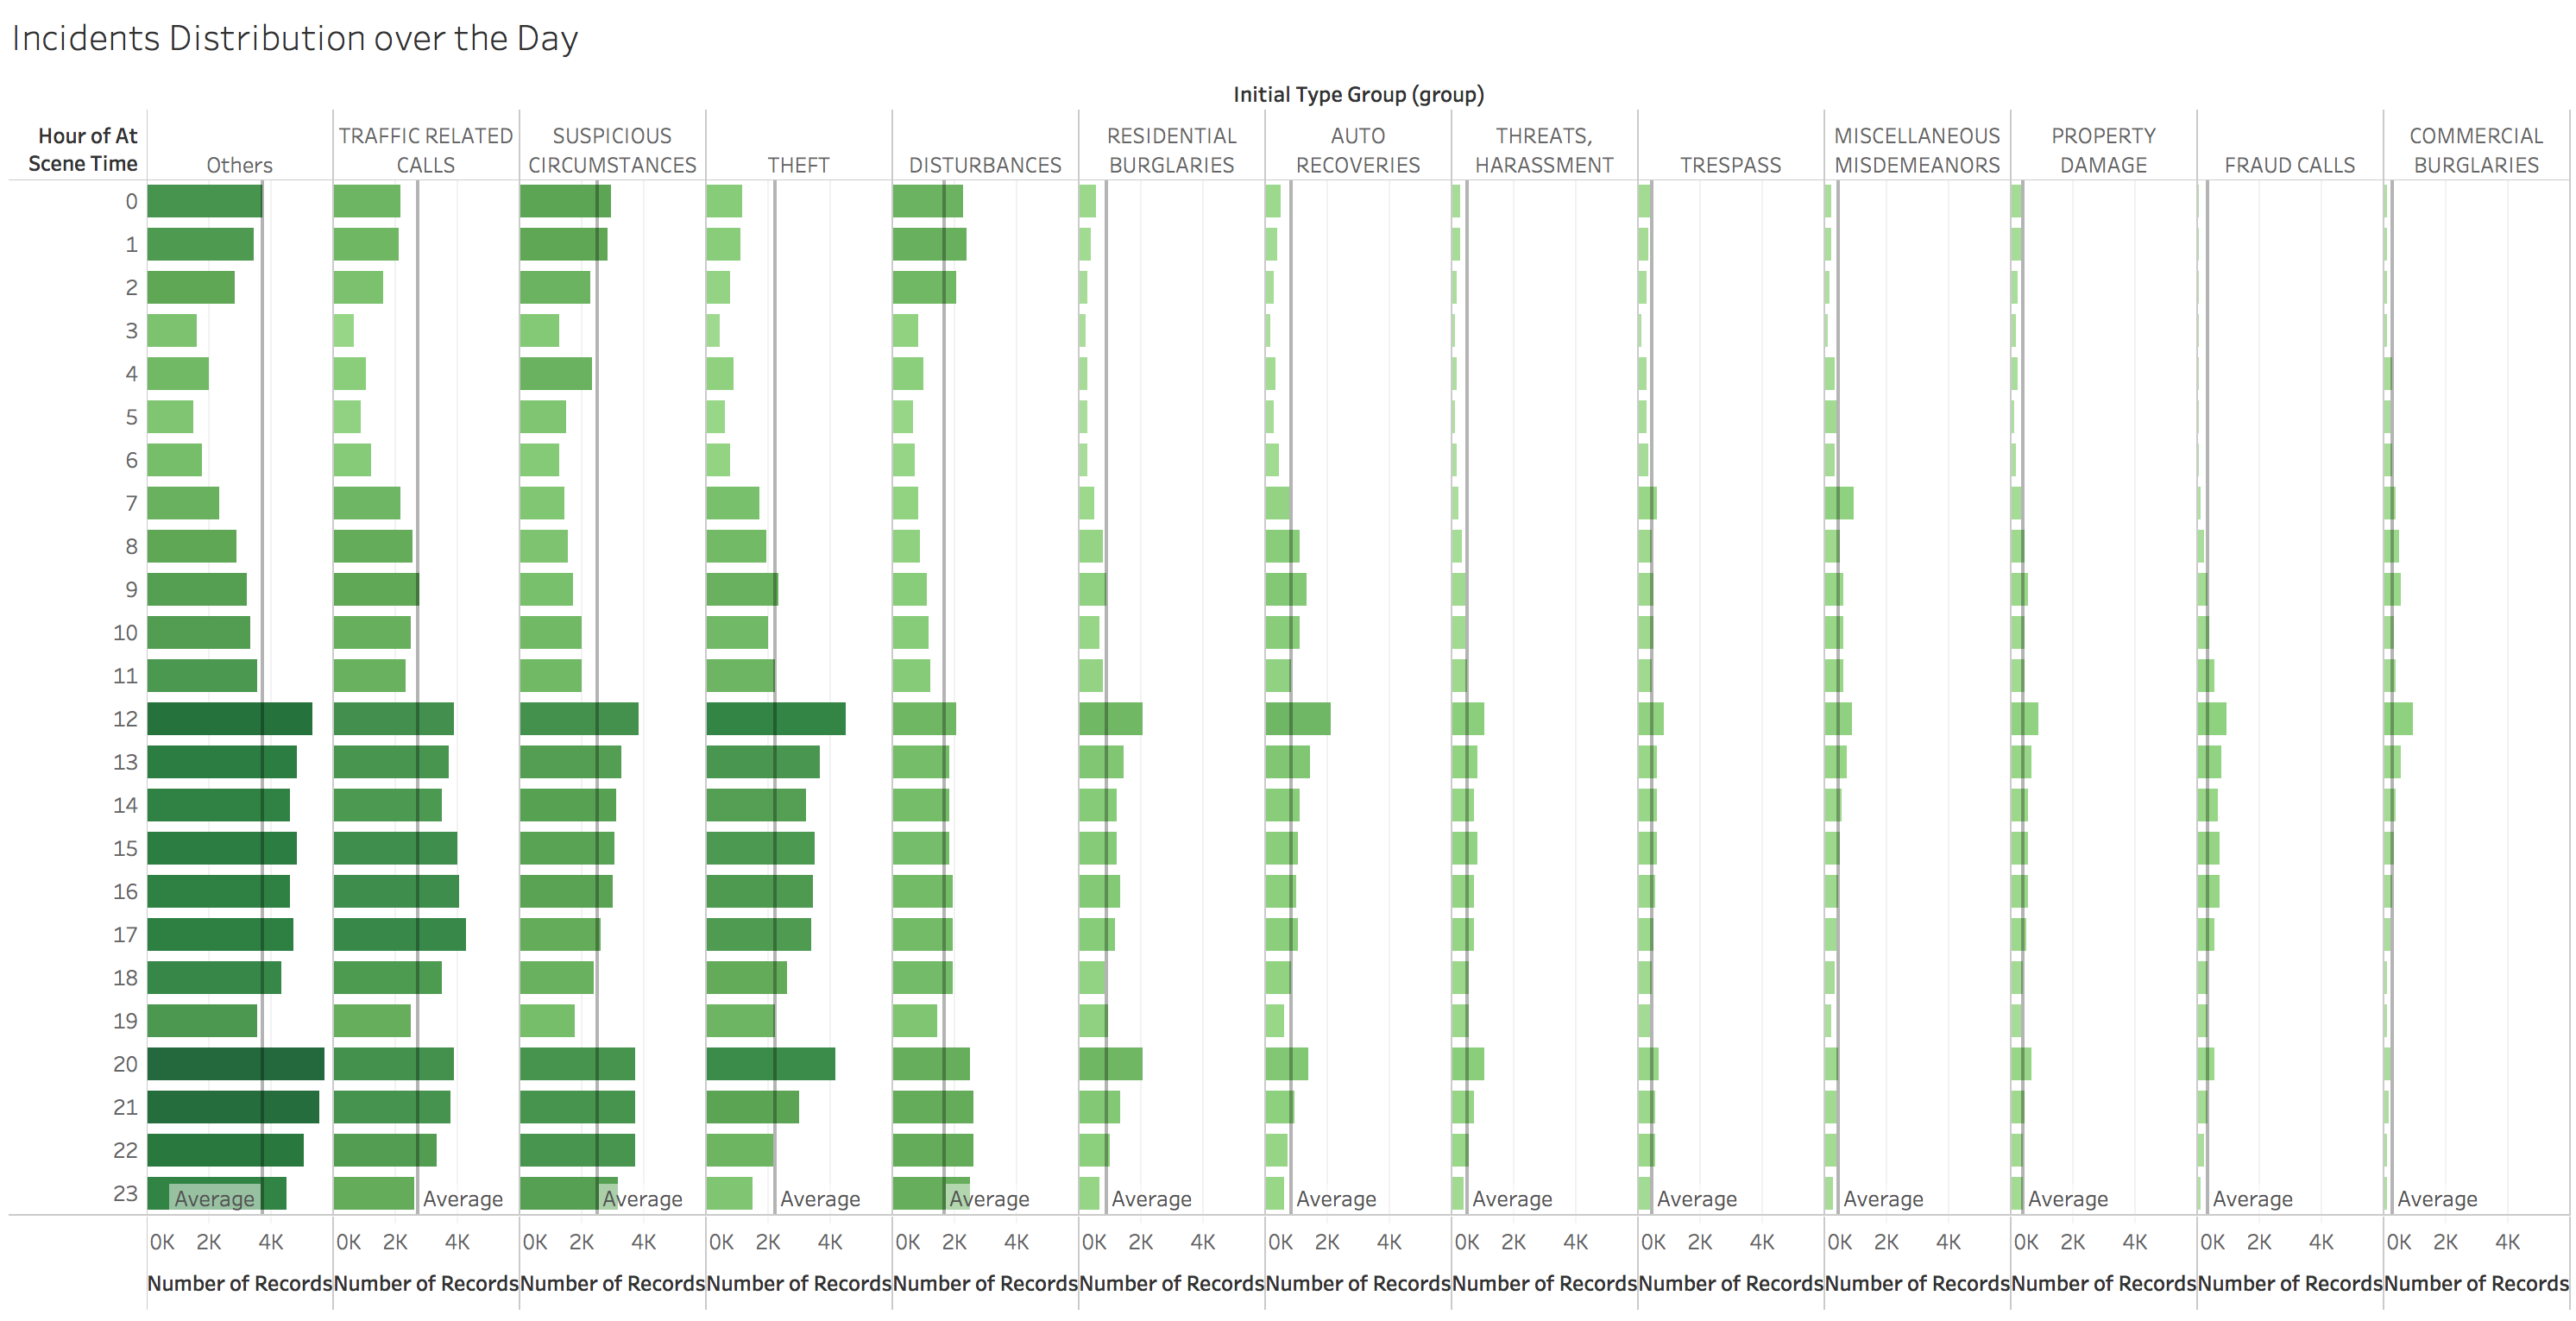
\includegraphics[width=\columnwidth]{figures/5_2_incidents_by_type_and_hour}
	\caption{Number of incidents by type over the different hours of the day. The sheet is called \textit{Incidents Distribution over the Day} in Tableau.}
	\label{fig:5_2_incidents_by_type_and_hour}
\end{figure}

From \cref{fig:5_2_incidents_by_type_and_hour} we can notice a common pattern among different types:
\begin{itemize}
	\item The number of incidents is generally smaller in the night / morning (23 - 11) and higher in the other hours.
	\item There are $2$ peaks, namely at $12$ and $20$: after these hours, incidents are still higher than the average but tend to gradually reduce in number.
	\item For most incidents the peaks have a similar number of incidents; there are a couple of exceptions, namely \textit{Fraud Calls} and \textit{Commercial Burglaries}, where the peak at $12$ is much higher than the one at $20$. 
\end{itemize}

\subsection*{Question 5.3}
\textit{How long does it take to clear incidents, as a function of the hour when they were reported? For example, do incidents reported at noon get cleared faster than incidents reported in the middle of the night?}

The visualization uses a bar chart.
The x-axis represents the hour of the day, while the y-axis shows the average resolution time for incidents reported in the given hour.
Color overloads the value showed in the y-axis.
The average line helps to compare particular time slots with the average behaviour.

Best practices for visualization suggests to use line charts instead of bar charts for continuous values like time.
In this case, however, we have discretized time into buckets of one hour and aggregated them together to compute the average.
In other words, we treat time as a discrete ordinal value.

\begin{figure}[h]
	\centering
	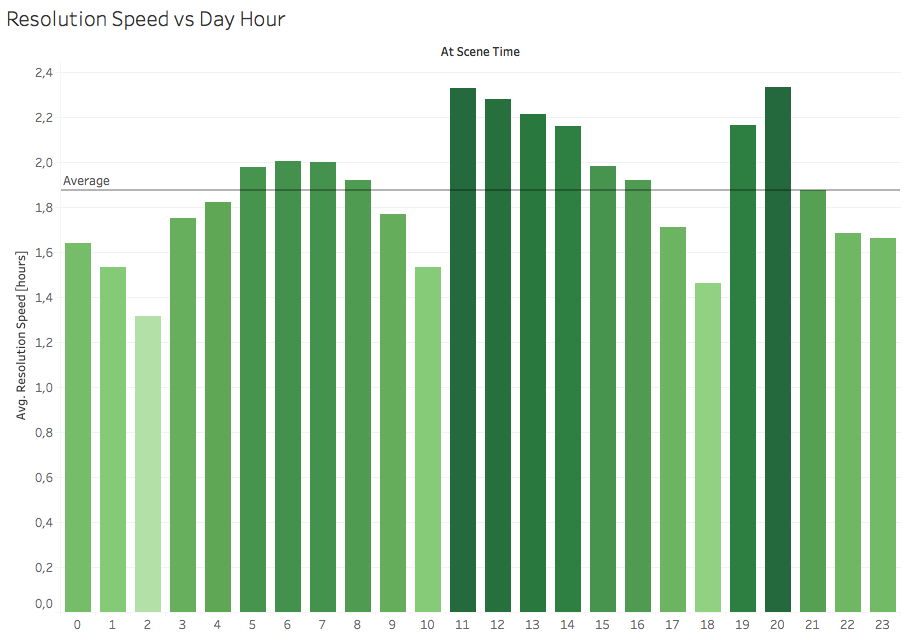
\includegraphics[width=0.9\columnwidth]{figures/5_3_resolution_speed_vs_hour}
	\caption{Resolution speed of incidents reported in different hour. The sheet is called \textit{Resolution Speed vs Day Hour} in Tableau.}
	\label{fig:5_3_resolution_speed_vs_hour}
\end{figure}

\cref{fig:5_3_resolution_speed_vs_hour} shows the visualization.
We can notice that:
\begin{itemize}
    \item The average time required to close incidents is not constant over the different hours of the day.
    \item Incidents that happens in the slots $11 - 14$ and $19 - 20$ take significant longer to be closed.
    \item Incidents that happens in the early morning ($5 - 7$) require on average more time than the incidents in the night and late morning ($9 - 10$).
    \item The time slots between $5 - 7$, $11 - 14$ and $19 - 20$ have a faster resolution speed.
\end{itemize}

To sum up, there is a correlation between the hour of the day and the time required to close incidents.
The visualization fully answers the question.

We have created a second visualization to check if this behaviour is common to all years.
The visualization uses again bar charts, one for each year.
The last column shows the average over all years as a reference for comparisons.
The axises are swapped in comparison to \cref{fig:5_3_resolution_speed_vs_hour} to better fit the screen.

\begin{figure}[h]
	\centering
	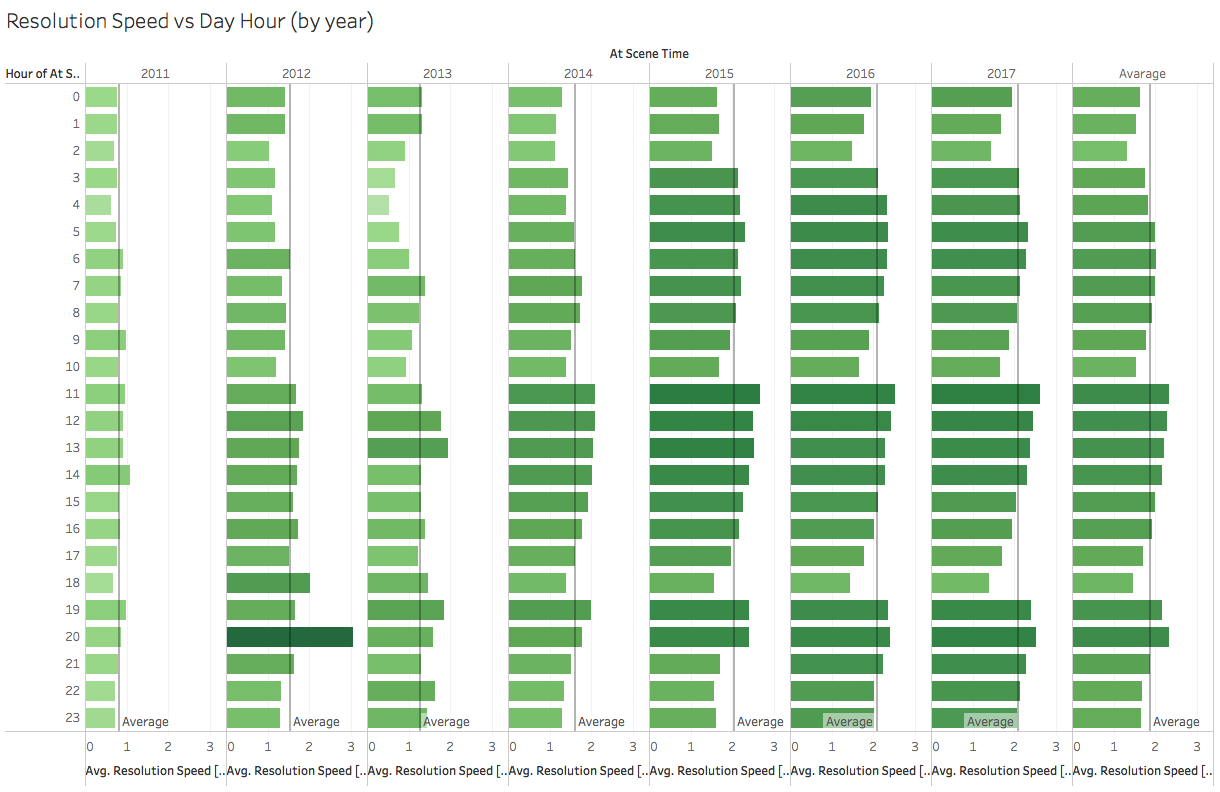
\includegraphics[width=0.9\columnwidth]{figures/5_3_resolution_speed_vs_hour_by_year}
	\caption{Resolution speed of incidents reported in different hour by year. The sheet is called \textit{Resolution Speed vs Day Hour (by year)} in Tableau.}
	\label{fig:5_3_resolution_speed_vs_hour_by_year}
\end{figure}

From \cref{fig:5_3_resolution_speed_vs_hour_by_year} we can notice that:
\begin{itemize}
    \item In $2011$ incidents are closed much faster than the average. There are some hours with a slightly higher resolution speed ($9$, $14$, $19$), but the difference with the rest of the day is small.
    \item Incidents that happens at $20$ in year $2012$ seems to take much longer to close than the average. This is probably due to the outliers discussed in \cref{sec:question3}, since both have very long resolution times and are in that slot of time.
    \item Years $2013$ have some picks in the slots $12 - 13$ and $18 - 20$. However, there are probably missing data for this year (see \cref{sec:question1}, so the confidence for this observation is low.
    \item Years $2014$, $2015$, $2016$ and $2017$ have a behaviour identical to the average over all years.    
\end{itemize}

To sum up, the resolution speed for the different hours of the day seems to be stable over years $2014$ to $2017$.
The previous years have slightly different behaviour, but still share some patterns.
Incidents that occurs in slots $5 - 7$, $11 - 14$ and $19 - 20$ take more time to be closed, while incidents between this slots are closed much faster.
